\documentclass[a4paper,11pt]{article}

% ConfigStream checkpoint report. This file intentionally reports the project
% at its current evidence boundary, rather than presenting unfinished work as
% a completed production evaluation.
\usepackage[a4paper,margin=2.5cm]{geometry}
\usepackage{setspace}
\usepackage{graphicx}
\usepackage{booktabs}
\usepackage{tabularx}
\usepackage{longtable}
\usepackage{array}
\usepackage{xcolor}
\usepackage{fancyhdr}
\usepackage{tikz}
\usetikzlibrary{calc}
\usepackage{enumitem}
% Keep the report buildable on the local MiKTeX installation when stringenc.sty
% is unavailable.
\IfFileExists{stringenc.sty}{\usepackage[hidelinks]{hyperref}}{\providecommand{\hypersetup}[1]{}}
\usepackage{natbib}

\onehalfspacing
\setlength{\parindent}{0pt}
\setlength{\parskip}{0.45em}
\setlist{topsep=0.25em,itemsep=0.15em}

\definecolor{ConfigBlue}{RGB}{0,56,101}
\definecolor{ConfigGray}{RGB}{80,88,96}
\definecolor{ConfigRed}{RGB}{194,31,48}
\definecolor{ConfigGold}{RGB}{190,145,50}
\hypersetup{
    colorlinks=true,
    linkcolor=ConfigBlue,
    urlcolor=ConfigBlue,
    citecolor=ConfigBlue,
    pdftitle={ConfigStream Checkpoint Report},
    pdfauthor={Nguyen Duc Dung; Pham Cong Hoang; Mai Vu Hoang; Le Tien Hop}
}

\pagestyle{fancy}
\fancyhf{}
\fancyhead[L]{\small\textbf{ConfigStream}}
\fancyhead[R]{\small Checkpoint report}
\fancyfoot[C]{\thepage}
\setlength{\headheight}{15pt}

\newcommand{\status}[1]{\textcolor{ConfigBlue}{\textbf{#1}}}
\newcommand{\metric}[1]{\textbf{#1}}

\begin{document}

\begin{titlepage}
\thispagestyle{empty}
\begin{tikzpicture}[remember picture,overlay]
  \draw[ConfigBlue,line width=2pt] ($(current page.north west)+(0.75cm,-0.75cm)$) rectangle ($(current page.south east)+(-0.75cm,0.75cm)$);
  \draw[ConfigGold,line width=0.8pt] ($(current page.north west)+(0.92cm,-0.92cm)$) rectangle ($(current page.south east)+(-0.92cm,0.92cm)$);
  \draw[ConfigGold,line width=2pt] ($(current page.north west)+(0.75cm,-1.55cm)$) -- ($(current page.north west)+(0.75cm,-0.75cm)$) -- ($(current page.north west)+(1.55cm,-0.75cm)$);
  \draw[ConfigGold,line width=2pt] ($(current page.north east)+(-1.55cm,-0.75cm)$) -- ($(current page.north east)+(-0.75cm,-0.75cm)$) -- ($(current page.north east)+(-0.75cm,-1.55cm)$);
  \draw[ConfigGold,line width=2pt] ($(current page.south west)+(0.75cm,1.55cm)$) -- ($(current page.south west)+(0.75cm,0.75cm)$) -- ($(current page.south west)+(1.55cm,0.75cm)$);
  \draw[ConfigGold,line width=2pt] ($(current page.south east)+(-1.55cm,0.75cm)$) -- ($(current page.south east)+(-0.75cm,0.75cm)$) -- ($(current page.south east)+(-0.75cm,1.55cm)$);
\end{tikzpicture}
\begin{center}
{\fontsize{16}{20}\selectfont\color{ConfigBlue}\textbf{HANOI UNIVERSITY OF SCIENCE AND TECHNOLOGY}\par}
\vspace{0.15cm}
{\fontsize{16}{20}\selectfont\textbf{School of Information and Communication Technology}\par}
\vspace{0.25cm}
\begin{tikzpicture}\draw[ConfigGold,line width=1.2pt] (0,0) -- (13.5,0);\fill[ConfigRed] (6.55,-0.06) rectangle (6.95,0.06);\end{tikzpicture}
\vspace{1.25cm}
{\fontsize{23}{28}\selectfont\color{ConfigBlue}\textbf{PROJECT REPORT}\par}
\vspace{0.15cm}
{\color{ConfigGold}\rule{7cm}{1pt}\par}
\vspace{0.3cm}
{\fontsize{22}{27}\selectfont\color{ConfigBlue}\textbf{ConfigStream}\par}
\vspace{0.18cm}
{\large\textbf{Version-aware configuration history, durable storage, and reproducible analytics}\par}
\vspace{0.25cm}
{\small\color{ConfigGray}\textbf{Checkpoint status through 25 October 2026}\par}
\vfill
\begin{minipage}{0.80\textwidth}
\renewcommand{\arraystretch}{1.15}
\begin{tabularx}{\linewidth}{@{}>{\bfseries}lX@{}}
Supervisor: & PhD Tran Viet Trung \\
\end{tabularx}
\end{minipage}
\vfill
\begin{minipage}{0.80\textwidth}
\small
\begin{tabularx}{\linewidth}{@{}>{\bfseries}X@{}}
\toprule
Member \\\midrule
Nguyen Duc Dung \\
Pham Cong Hoang \\
Mai Vu Hoang \\
Le Tien Hop \\
\bottomrule
\end{tabularx}
\end{minipage}
\vspace{0.55cm}
{\color{ConfigGold}\rule{5cm}{0.8pt}\par}
\vspace{0.15cm}
{\large\color{ConfigBlue}\textbf{Ha Noi, 2026}\par}
\end{center}
\end{titlepage}

\pagenumbering{roman}
\tableofcontents
\clearpage
\listoftables
\clearpage
\listoffigures
\clearpage

\section*{List of Abbreviations}
\addcontentsline{toc}{section}{List of Abbreviations}
\begin{tabularx}{\textwidth}{@{}p{0.22\textwidth}X@{}}
    API & Application Programming Interface \\
    DNS & Domain Name System \\
    HA & High Availability \\
    IaC & Infrastructure as Code \\
    JSONL & JSON Lines \\
    RPKI & Resource Public Key Infrastructure \\
    RIS & Routing Information Service \\
    SUT & System Under Test \\
\end{tabularx}
\clearpage

\pagenumbering{arabic}

\section{Checkpoint scope and status}

This report records the state of ConfigStream through 25 October 2026. It reports implemented components, accepted evidence, pending experiments, and claims that remain outside the tested scope. The date defines the evidence boundary; the report does not convert project progress into a percentage.

The central question is whether a streaming system can preserve enough identity, event-time information, provenance, and validation evidence to support trustworthy configuration-history analysis. ConfigStream addresses this question by combining Kafka ingestion, stateful Spark Structured Streaming, authoritative Parquet history in MinIO, rebuildable search projections, and a read-only API/dashboard. The design makes a deliberate separation between the historical record and the indexes used to browse it.

By this date, the implementation path, the main lake-first publication path, and several correctness and replay artifacts are available. Remaining work concerns comparative evaluation, failure and recovery coverage, reproducibility packaging, and final alignment between evidence and claims.

\begin{table}[ht]
\centering
\caption{Checkpoint status by work package.}
\label{tab:checkpoint-status}
\begin{tabularx}{\textwidth}{@{}p{0.27\textwidth}p{0.16\textwidth}X@{}}
\toprule
Work package & Status & Evidence boundary \\
\midrule
Data contracts and workload generation & Complete & Versioned asset/snapshot/event contracts and domain-specific workload artifacts are present. \\
Streaming ingestion and state & Complete for current scope & Kafka-to-Spark processing, event-time buffering, deduplication, adjacent-version pairing, and diagnostics are implemented. \\
Historical storage and projections & Complete for current scope & MinIO/Parquet is treated as authoritative; Elasticsearch and the API are rebuildable read paths. \\
Dashboard and evidence views & Accepted & The Phase 20V read-only views expose history, aggregates, experiments, and evidence details. \\
Correctness and replay evaluation & Substantially complete & TerraDS replay and the corrected 27-trial matched campaign have accepted artifacts. \\
Production-scale and HA evaluation & Pending & Full paced RIS capacity, H3, multi-node HA, and end-to-end exactly-once evidence remain outside the current claim. \\
\bottomrule
\end{tabularx}
\end{table}

\section{Problem and research questions}

Configuration history is easy to store incorrectly. A system that compares the previous message with the current message can silently construct the wrong transition when messages arrive out of order. A search index can make a result look available while the authoritative history is incomplete. A throughput number can also be misleading when one workload reports rows per second and another reports occurrences, files, or bytes.

ConfigStream therefore treats a configuration change as a provenance-bearing temporal record. A change is meaningful only when the system can identify the asset, order versions using the producer's version semantics, reconstruct adjacent states, and retain enough evidence to reproduce the resulting diff or alert.

The checkpoint evaluates three research questions:

\begin{enumerate}
    \item \textbf{RQ1:} Can ConfigStream reconstruct adjacent configuration states correctly under out-of-order arrival, duplicates, bounded buffering, and restart-sensitive streaming execution?
    \item \textbf{RQ2:} Does a lake-first storage boundary preserve a trustworthy historical record while allowing search and API projections to be rebuilt independently?
    \item \textbf{RQ3:} How should correctness, throughput, latency, storage growth, and resource use be measured across workloads whose units and semantics are different?
\end{enumerate}

The current evidence answers the implementation portion of these questions positively for the tested scope. It does not yet support claims about cluster-wide scalability, HA, or universal configuration parsing.

\section{System design}

\subsection{Architecture at a glance}

Figure~\ref{fig:architecture} summarizes the architecture in the form used for the paper. The figure separates four ideas that are often mixed together in an engineering diagram: the typed record entering the system, the event-time state transition, the publication boundary, and the evidence-aware evaluation loop.

\begin{figure}[ht]
    \centering
    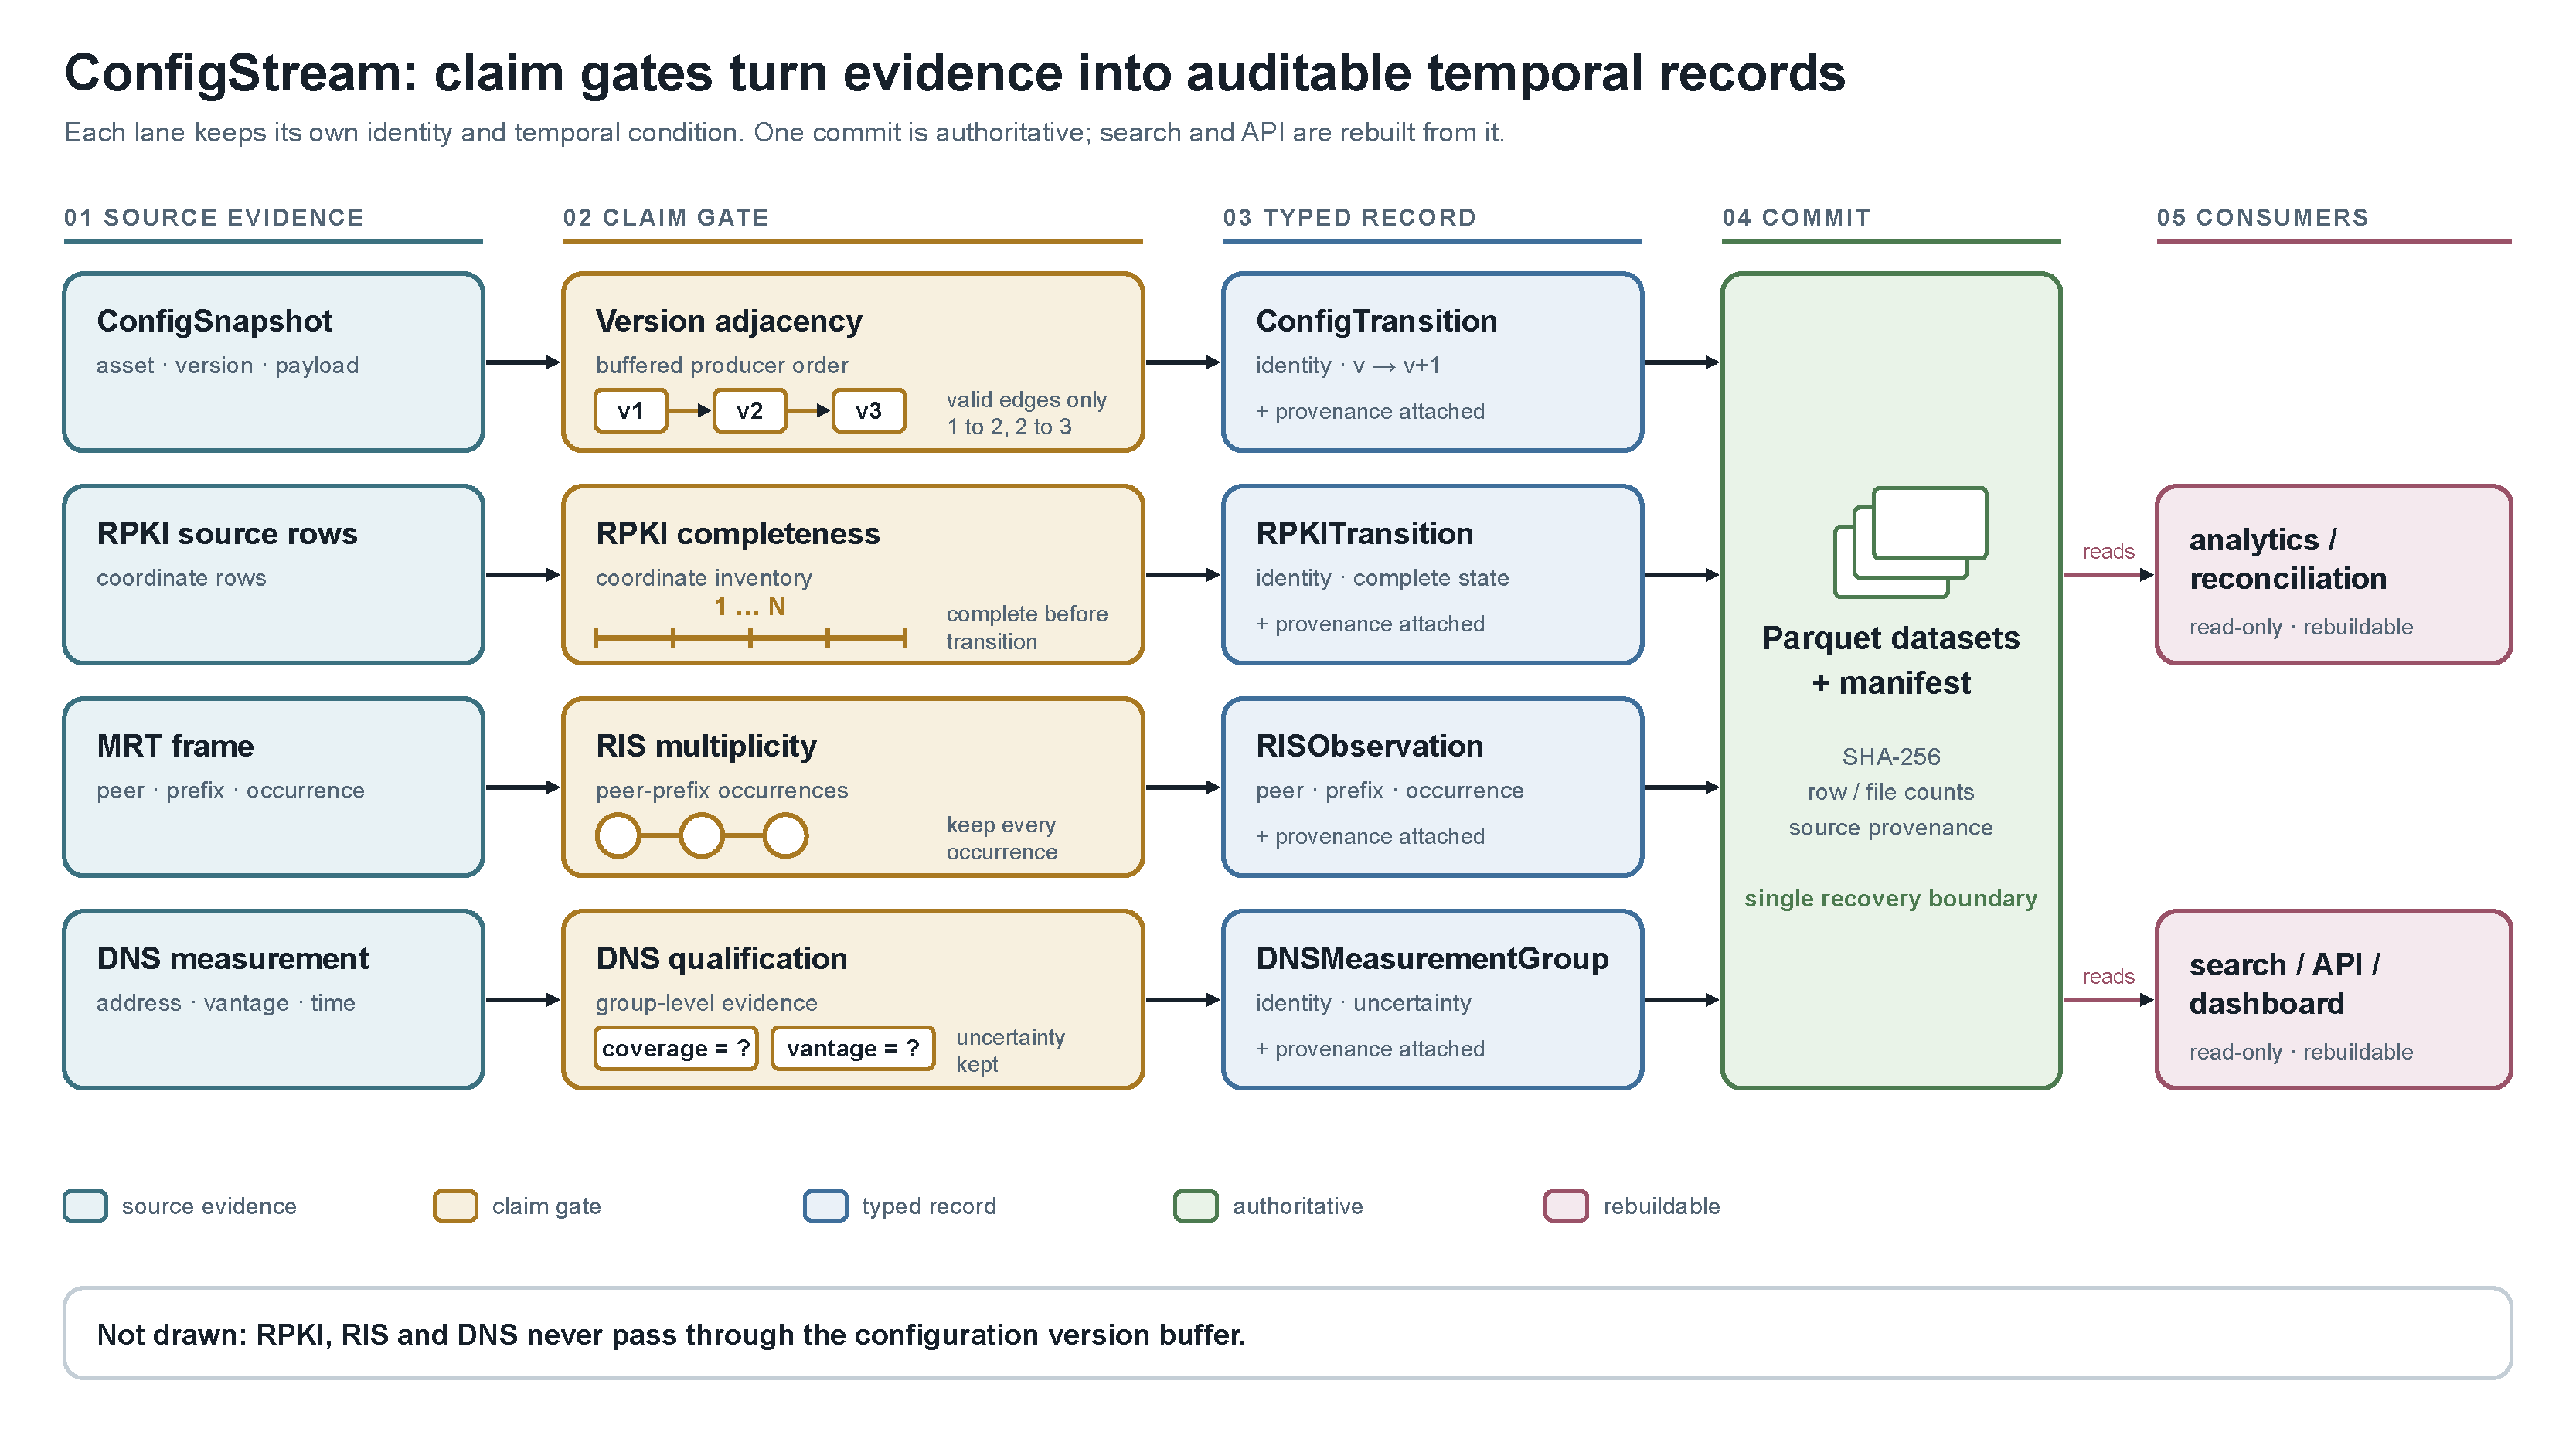
\includegraphics[width=\textwidth]{figures/configstream-platform-architecture.pdf}
    \caption{ConfigStream evidence flow. Source-specific gates create typed temporal records, the manifest defines the authoritative commit, and downstream views remain rebuildable.}
    \label{fig:architecture}
\end{figure}

The implemented path is:

\begin{enumerate}
    \item a source or generator publishes typed snapshots to Kafka, keyed by \texttt{asset\_id};
    \item Spark Structured Streaming validates records, applies event-time watermarks and identifier deduplication, and maintains bounded per-asset state;
    \item the processor pairs adjacent producer versions, normalizes the two states, computes a deterministic diff, evaluates configured rules, and emits diagnostics when state is incomplete;
    \item the commit boundary writes authoritative history and derived evidence to MinIO/Parquet;
    \item Elasticsearch, FastAPI, and the dashboard expose rebuildable metadata and read-only views for inspection.
\end{enumerate}

\subsection{State and pairing policy}

The system consumes \texttt{config.snapshots} for core state reconstruction. It does not rely on the arrival order of \texttt{config.events}, and it does not require the \texttt{config.assets} topic to compute the core diff. For each asset, the processor keeps a bounded version buffer. After sorting by the producer-defined version field, it compares adjacent versions, not merely consecutive arrivals. A record that arrives late can therefore complete a transition that would be invalid under an arrival-order implementation.

The code stores the version in \texttt{ConfigSnapshot.version} as a producer-assigned integer. The notation v1, v2, and v3 below is an example, not a fixed dataset convention. For arrival order v1, v3, v2, the buffer first retains [v1,v3] and emits no adjacent edge. When v2 arrives within the retention policy, the sorted state is [v1,v2,v3] and the processor emits v1--v2 and v2--v3. It does not emit v1--v3 as an adjacent streaming transition. The pure comparison helper can accept non-consecutive endpoints and report a version gap; that separate API boundary must not be confused with the streaming emission rule.

The buffer is intentionally bounded. When a version gap, eviction, duplicate, or malformed record prevents a complete transition, the system records a diagnostic rather than inventing a diff. This choice makes incompleteness visible and keeps the correctness contract explicit. The default policy retains at most 32 versions per asset, applies a ten-minute event-time watermark delay, and clears inactive state after a 30-minute event-time timeout. The accepted TerraDS replay used its registered run settings, which must be reported separately from these defaults.

\subsection{Common evidence contract}

The common contract layer gives every record an identity, a time interpretation, and a provenance reference. A \texttt{ConfigSnapshot} carries \texttt{snapshot\_id}, \texttt{asset\_id}, producer version, event time, ingest time, and a raw content hash. Source-specific temporal records carry the corresponding source coordinate and manifest reference. A record identity is derived from canonical fields and a named policy; it is not inferred from a Kafka offset or from the order in which a consumer sees messages.

This distinction determines what the system can safely claim. A repeated delivery with the same logical identity can be suppressed or reconciled. A second record that reuses an identity with different content is a conflict. A timestamp identifies when an observation was made, but it does not establish which producer version precedes another. The processing code therefore keeps identity, producer order, event time, and transport provenance as separate fields.

\subsection{Configuration transformation}

Only an admitted adjacent pair enters the configuration transformation. The normalizer converts supported text into a deterministic line representation, applies the implemented whitespace and generated-comment rules, and masks selected secret-like settings. It produces a normalized hash while preserving the raw hash of the source bytes. These hashes answer different questions: the raw hash identifies the received content, while the normalized hash identifies the content under the declared policy.

The diff compares normalized lines with deterministic line-based logic. The result identifies the old and new snapshots, their versions, the policy, and the normalized hashes. YAML rules inspect the normalized diff and create deterministic alerts. The method supports the registered text representation. It is not a vendor-aware configuration parser, a complete secret detector, or proof that a proposed change is safe to deploy.

\subsection{Source-specific temporal lanes}

RPKI, RIS, and DNS do not pass through the configuration version buffer. They share the evidence contract and the publication boundary, but each lane has its own identity and completion condition.

\paragraph{RPKI.}
The RPKI path decodes source chunks into canonical authorization rows and records their source coordinates. A daily state is eligible for comparison only when the expected coordinate inventory is complete, the source manifest and artifact digest validate, and the accepted-row count and state digest agree with the observation descriptor. A transition compares two compatible consecutive complete states. An incomplete daily input remains incomplete; the processor does not infer deletions from rows that have not been observed.

\paragraph{RIS.}
The RIS path frames MRT input and projects records into peer-prefix occurrences. Occurrence identity retains the frame and record coordinate. Repeated observations are not collapsed into a set because multiplicity is part of the evidence. The resulting record answers an occurrence-processing question. It does not claim to be a complete global BGP state or a count of unique deployed routes.

\paragraph{DNS.}
The DNS path groups measurements by the declared query, response, address, and vantage dimensions. It carries coverage and vantage uncertainty into the output. A qualified difference requires the declared comparison policy and the required partition or group completeness. An unknown coverage or vantage value remains unknown; the implementation does not turn it into evidence of global disappearance.

\subsection{Publication and recovery}

The publication boundary is lake-first. A batch writes raw provenance and typed processed records to Parquet, inventories the files, validates byte counts and row counts, computes or checks SHA-256 values, and writes a manifest only after the expected data is present. Readers use the manifest to exclude partial or uncommitted batches.

Search, FastAPI, and the dashboard are derived projections. If a projection is missing or stale, recovery reads the committed Parquet datasets, rebuilds the projection, and reconciles logical identities and counts. A failed projection does not change the authoritative history. The boundary does not make Kafka, Spark, MinIO, and Elasticsearch one distributed transaction, so the report does not claim end-to-end exactly-once processing.

\subsection{Evaluation method}

The evaluation follows the same boundaries as the implementation. Configuration replay checks snapshot identity, adjacent-pair identity, normalized output, alert identity, diagnostics, lake contents, and manifest integrity. RPKI checks complete-state membership, digests, transition equality, storage layout, and query equality. RIS checks framed occurrence identity and multiplicity. DNS checks qualified groups while retaining coverage and vantage fields.

Every performance result keeps its workload unit and processing boundary. TerraDS reports snapshots and adjacent pairs for an end-to-end replay. The matched B0/B2/B3 campaign compares one normalized projection under fresh processes and excludes source parsing and production state finalization. RPKI, RIS, and DNS rates are not pooled. This separation is part of the method because a row, an occurrence, a file version, and a measurement group do not represent the same object.

\subsection{Normalization, diff, and publication}

Normalization is deterministic and line-oriented for the supported configuration representation. The system retains a raw hash and a normalized hash, which lets the evaluator distinguish byte-level changes from semantic changes under the chosen normalization policy. Selected secret-like keys are masked according to the implemented rule set. The current method should not be described as a universal parser or a universal secret detector.

The publication rule is lake-first. A commit manifest records the relationship between authoritative Parquet artifacts and rebuildable projections. If Elasticsearch or the dashboard is unavailable, the historical record remains the recovery source. This design does not remove all failure modes, and it does not justify an end-to-end exactly-once claim. It does define where correctness must be checked first.

\section{Current experimental evidence}

\subsection{Evidence roles and workload semantics}

The evaluation uses distinct workloads for distinct questions. TerraDS represents a configuration-history replay with files and adjacent versions. RPKI, DNS, and RIS exercise processing paths with different record units and temporal structure. Their rates are not pooled into a single headline number.

\begin{table}[ht]
\centering
\caption{Accepted workload evidence at the checkpoint.}
\label{tab:workloads}
\small
\begin{tabularx}{\textwidth}{@{}p{0.14\textwidth}p{0.16\textwidth}p{0.18\textwidth}p{0.20\textwidth}X@{}}
\toprule
Workload & Main unit & Input size & Change/transition evidence & Interpretation \\
\midrule
TerraDS & file/version & 375 repositories, 10,188 versions & 3,683 adjacent pairs and 12,278,085 logical bytes & End-to-end configuration-history replay \\
RPKI & canonical row & 5,062,923 repeated tuples & 12,016 additions/removals & Large row-oriented batch path \\
DNS & row/address group & 2,234,863 rows & 4,091 changes among 144,883 common groups & Grouped temporal comparison \\
RIS & peer-prefix occurrence & 4,725,156 occurrences & Source characterization retained separately & Stream-like occurrence workload; full paced capacity remains pending \\
\bottomrule
\end{tabularx}
\end{table}

\subsection{End-to-end TerraDS replay}

The accepted TerraDS replay processed 10,188 snapshots and formed 3,683 adjacent diffs. It committed 29,402,997 raw and processed Parquet bytes, emitted zero alerts and zero diagnostics, and completed after the publisher drained in 68.742 seconds. The publisher rate was 500.023 snapshots/s. The accepted logical rate, which includes the workload's logical-byte interpretation, was 148.205 snapshots/s.

These numbers demonstrate an end-to-end path under the accepted replay conditions. They do not establish a production capacity limit. A supplemental headroom replay used the same history and pairs but produced 29,346,912 Parquet bytes and 139.565 accepted snapshots/s; because the runs were not a matched comparison, the difference should not be presented as a model improvement.

\subsection{Corrected matched processing campaign}

The corrected campaign contains 27 exact trials: nine configurations with three fresh-process repetitions each. The compared B0, B2, and B3 modes produced identical full normalized rows in all accepted trials. B3 also reported zero selected-offset lag. The table reports medians with observed ranges in seconds.

\begin{table}[ht]
\centering
\caption{Matched processing medians and observed ranges.}
\label{tab:matched}
\small
\begin{tabular}{@{}lccc@{}}
\toprule
Workload & B0 & B2 & B3 \\
\midrule
RPKI (360,226 rows) & 6.297 (6.282--12.577) & 16.840 (14.729--21.080) & 25.417 (23.144--25.424) \\
RIS (370,141 occurrences) & 10.485 (8.437--12.636) & 21.167 (18.967--23.186) & 29.644 (23.233--29.726) \\
DNS (4,096 rows) & 2.089 (2.087--6.302) & 10.536 (10.486--12.584) & 16.866 (12.624--16.924) \\
\bottomrule
\end{tabular}
\end{table}

The matched result supports a narrow conclusion: under the tested normalized-core workload, the modes agree on output while incurring different processing times. The result excludes production-specific parsing, state finalization, and full production ranking. It is therefore a component comparison, not a claim that one mode is universally superior.

\subsection{Storage and resource observations}

The matched campaign produced 1,622,766,994 Parquet bytes and 1,623,023,143 MinIO namespace bytes. Retained growth was 3,869,485,576 bytes, below the amended 6 GiB limit. The peak tree was 1,612,824,576 bytes, the minimum observed guest RAM was 4,191,440,896 bytes, and no resource failure occurred. The aggregate processing time was 502.981 seconds, below the 7,200-second acceptance limit.

The initial pilot failed because a SQLite connection was used from the wrong Spark callback thread. That attempt produced zero committed files and is retained as a failed trial. The corrected retry passed. Reporting both attempts matters because the failure identifies a real integration boundary rather than an unexplained missing result.

\section{What is complete and what remains}

\subsection{Completed at the checkpoint}

\begin{itemize}
    \item The core data contracts, topic boundaries, and asset-keyed ingestion path are defined.
    \item The streaming processor implements event-time buffering, deduplication, adjacent-version pairing, deterministic normalization, diffing, alert evaluation, and diagnostics.
    \item MinIO/Parquet provides the authoritative historical path, while the search/API layer is treated as a rebuildable projection.
    \item A Kubernetes single-node acceptance run covers the real Kafka-to-Spark-to-MinIO path for the current deployment scope.
    \item The read-only dashboard exposes historical and experimental evidence rather than mutable operational controls.
    \item TerraDS replay and the corrected matched campaign provide auditable evidence with explicit acceptance boundaries.
\end{itemize}

\subsection{Not yet complete}

The project has not completed a full paced RIS capacity comparison, the H3 branch, a multi-node high-availability deployment, or a failure campaign that establishes recovery guarantees under realistic component loss. The current artifacts also do not justify an end-to-end exactly-once claim. These are evaluation gaps, not implementation details that can be silently inferred from the successful replays.

The paper still needs a final human pass over hardware and operating-system metadata, reference formatting, author contributions, data/code availability, and the exact relationship between each table and its source artifact. Those items are part of the path from an accepted checkpoint to a submission-ready report.

\section{Risk assessment}

\begin{table}[ht]
\centering
\caption{Main risks and mitigation actions.}
\label{tab:risks}
\begin{tabularx}{\textwidth}{@{}p{0.25\textwidth}p{0.25\textwidth}X@{}}
\toprule
Risk & Why it matters & Mitigation for the next checkpoint \\
\midrule
Overclaiming scalability & Single-node acceptance cannot represent cluster capacity or HA. & Report deployment scope explicitly and run a matched multi-node or paced-load study if the claim is required. \\
Mixed workload units & Rows, occurrences, files, and bytes answer different questions. & Keep a workload-role matrix and report denominators next to every rate. \\
Projection drift & Search results can diverge from authoritative history. & Add manifest-based reconciliation and a documented rebuild test. \\
Late or missing state & A bounded buffer can evict a version before its predecessor arrives. & Expand adversarial out-of-order tests and publish diagnostic counts by reason. \\
Reproducibility gaps & A result without environment and artifact provenance is hard to audit. & Freeze run manifests, hardware metadata, seeds, and exact command lines. \\
\bottomrule
\end{tabularx}
\end{table}

\section{Next steps }

The next phase should reduce uncertainty rather than add more components. The recommended order is:

\begin{enumerate}
    \item \textbf{Close the evidence ledger.} Attach every reported number to a run manifest, environment record, artifact path, and acceptance criterion. Record the exact hardware and operating-system details.
    \item \textbf{Finish the deferred comparisons.} Run the approved paced RIS experiment and H3 only if their hypotheses and denominators are fixed in advance. Keep them separate from the accepted matched campaign.
    \item \textbf{Test recovery and projection rebuild.} Delete or make unavailable a rebuildable projection, reconstruct it from Parquet and the manifest, and verify row counts, hashes, and query results. Then document the limits of the recovery guarantee.
    \item \textbf{Expand correctness tests.} Add adversarial cases for duplicate identifiers, late versions, version gaps, buffer eviction, malformed records, and restart boundaries. Check both positive diffs and diagnostics.
    \item \textbf{Prepare the final presentation.} Use one architecture figure, one state-reconstruction example, one evaluation table, one evidence dashboard view, and one limitations/next-steps slide. Avoid a service inventory as the main story.
\end{enumerate}

\begin{table}[ht]
\centering
\caption{Milestones after the 25 October 2026 evidence boundary.}
\label{tab:roadmap}
\begin{tabularx}{\textwidth}{@{}p{0.16\textwidth}p{0.31\textwidth}X@{}}
\toprule
Milestone & Deliverable & Exit condition \\
\midrule
M1 & Reproducible evidence pack & Every accepted result has a manifest, environment, command, output artifact, and reviewer-readable interpretation. \\
M2 & Deferred evaluation and recovery & RIS/H3 decisions are documented; projection rebuild and adversarial state tests pass or are explicitly bounded. \\
M3 & Final paper and talk & Claims, figures, tables, references, and speaker narrative agree with the evidence ledger. \\
\bottomrule
\end{tabularx}
\end{table}

\section{Conclusion}

At the checkpoint, ConfigStream is a functioning evidence-oriented prototype with a substantially complete implementation path and accepted replay results. Its strongest current contribution is the separation of temporal state reconstruction, authoritative history, and rebuildable read projections. Its strongest limitation is the narrow deployment and evaluation envelope. The next report should therefore focus on closing evidence gaps and tightening claims, not on presenting the current single-node results as a general scalability result.

\nocite{*}
\bibliographystyle{plainnat}
\bibliography{../../docs/configstream_references}

\end{document}
